\documentclass{article}
\usepackage[margin=0.8in]{geometry} % change this parameter to enlarge/restrict the margins
\usepackage{amsmath,amsthm,amssymb,amsfonts, fancyhdr, color, comment, graphicx, environ}
\usepackage{xcolor}
\usepackage{mdframed}
\usepackage[shortlabels]{enumitem}
\usepackage{hyperref}
\usepackage{calrsfs}
\DeclareMathAlphabet{\pazocal}{OMS}{zplm}{m}{n}
\usepackage{graphicx}
\usepackage{makecell} %table cells
\usepackage{booktabs} %table appearance
\usepackage{caption} %table caption

\renewcommand{\footrulewidth}{0.8pt}
\hypersetup{
	colorlinks=true,
	linkcolor=blue,
	filecolor=magenta,      
	urlcolor=blue,
}

%/ Margin
%/ ##########################
%/\addtolength{\oddsidemargin}{-.7in}
%/\addtolength{\evensidemargin}{-.7in}
%/\addtolength{\textwidth}{1.4in} %/Double of the 2 above
% ###########################

% fancy style 
\pagestyle{fancy}
% remove fancy style from bottom 
\renewcommand{\footrulewidth}{0pt}

\lhead{Group 20}
\rhead{Algorithmic Machine Learning} 

\newcommand{\loss}{L(\theta, a)}
\newcommand{\lossRule}{L(\theta, \delta(x))}
\newcommand{\risk}{R(\theta, \delta)}

%------------------------------------------------
% Bibliography
\usepackage[sorting=none, backend=bibtex]{biblatex}
\addbibresource{ref.bib}
%------------------------------------------------


\begin{document}
	\title{\Large Algorithmic Machine Learning  \\[0.5cm]
	\bf\Large Challenge 1 - Report \\[0.5cm]
	
	\bf\Large Group 20}

\author{\large 
	\begin{tabular}{rl}
		\textbf{Professor:} & Pietro Michiardi \\
		\textbf{Authors:} & Daniele Falcetta \\ & Simone Papicchio \\ & Massimiliano Pronesti \\ & Federico Tiblias
	\end{tabular}
	}
\date{\large \today}

\makeatletter
\begin{titlepage}
	\begin{center}
		{ 
\includegraphics[width=10cm]{assets/eurecom.png}}
		{\ \\ \ \\}
		\vbox{}\vspace{5cm}
		{\@title }\\[3cm]
		{\@author}\\[3cm]
		{\@date\\}
		
	\end{center}
\end{titlepage}
\makeatother
	
\section{Introduction}


    Anomalous sound detection (ASD) is the task to identify whether the sound emitted from a target machine is normal or anomalous. Automatically detecting mechanical failure is an essential technology in the fourth industrial revolution, including artificial intelligence (AI)-based factory automation. Prompt detection of machine anomaly by observing its sounds may be useful for machine condition monitoring.

    The main challenge of this task is to detect unknown anomalous sounds under the condition that only normal sound samples have been provided as training data. In real-world factories, actual anomalous sounds rarely occur and are highly diverse. Therefore, exhaustive patterns of anomalous sounds are impossible to deliberately make and/or collect. This means we have to detect unknown anomalous sounds that were not observed in the given training data. We are given sound samples of different machines along with their IDs, and want to build a model which can be used to predict whether an unknown sound (this unknown sound belongs to one of the given machine IDs in the training dataset) is normal or anomalous. Rather than a clustering or discriminative approach, this challenge calls for a generative solution able to infer a distribution for normal samples and give a likelihood score for a test datapoint.
    
    We try different approaches starting from simpler Machine Learning and clustering techniques such as PCA with KDE and DBSCAN to more complex ones like f-ANOGAN, Linear and Convolutional Autoencoders and SVDD.


\section{Data Analysis \& Pre-processing}
    \subsection{Data exploration}
    The data used for this task comprises parts of ToyADMOS and the MIMII Dataset consisting of the normal/anomalous operating sounds of six types of toy/real machines. Each recording is a single-channel (approximately) 10-sec length audio that includes both a target machine's operating sound and environmental noise. In this work, we work on only one machine type (i.e. Slide rail). 
    In this section we describe all the different preprocessings we used.
    
    \subsection{Outlier detection}
	While the dataset clearly differentiates between normal and anomalies, we cannot be certain that the training set does not contain outliers.
	A brief analysis in both time and frequency domain suggests this is not the case. There are no features that present anomalous characteristics and PCA reveals no visible outliers. No samples were discarded at this stage.
	
   	\subsection{Transformations}
   	Different transformations are applied for different experiments. 
	\begin{itemize}
		\item \textbf{Fast Fourier Transform:} Scipy's \texttt{fft} is applied on the whole audio track. This is a fast and straightforward transformation that is worth exploring in conjunction with classical machine learning models.
		\item \textbf{PCA:} Provides fast dimensionality reduction which can prove useful when fitting models suffering from curse of dimensionality.
		\item \textbf{Log Mel Spectrogram:} librosa's \texttt{melspectrogram} produces a 2D output by performing a Fourier Transform on different parts of the sample with a rolling window approach. The output is then rescaled using a log transformation. This results in an image which can be used in more refined deep-learning models.
	\end{itemize}
    
    \subsection{Denoising}
     For this point we decide to use the noisereduce \cite{tim_sainburg_2019_3243139} library, based on a noise reduction algorithm in python that reduces noise in time-domain signals like speech, bioacoustics, and physiological signals. It relies on a method called "spectral gating" which is a form of Noise Gate \cite{sainburg2020finding}. It works by computing a spectrogram of a signal and estimating a noise threshold (or gate) for each frequency band of that signal/noise. That threshold is used to compute a mask, which gates noise below the frequency-varying threshold. In this work we try different noise reduction proportion values.
     \begin{figure}
        \centering
        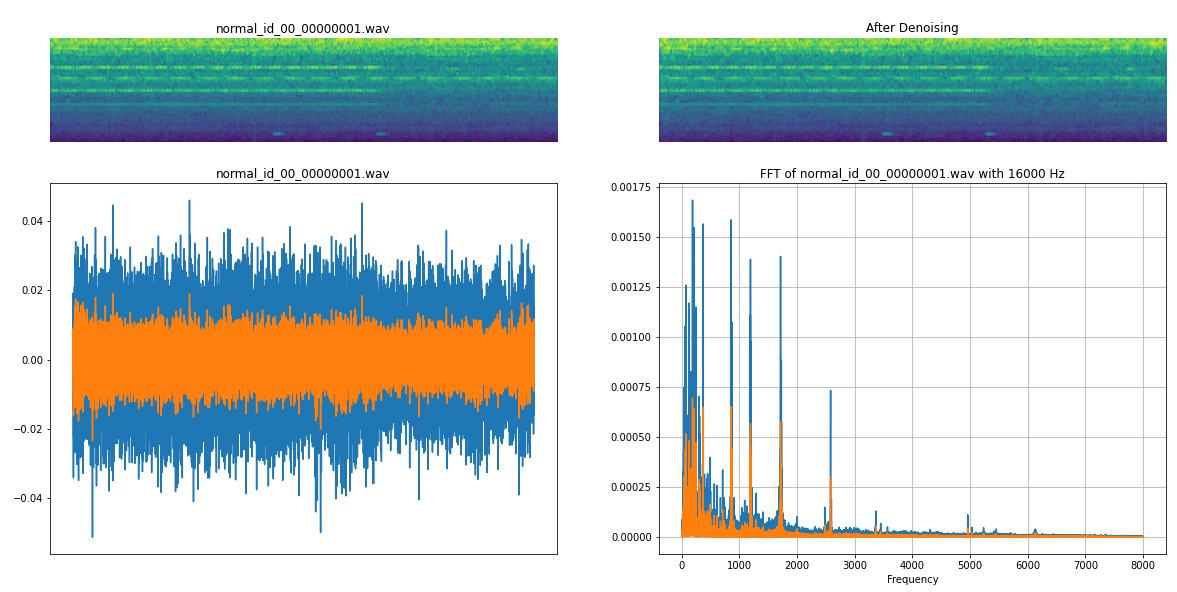
\includegraphics[width=\linewidth]{assets/mod_out_normal_id_00_00000001.wav.png}
        \caption{The log mel spectrograms for a not anomalous sample before and after denoising, with a reduction rate of 0.6. Below the plots of the .wav signal and his FFT, both before (blue) and after (orange) denoising}
        \label{fig:normal_id_denos}
    \end{figure}


\section{Models}
We try different approaches to tackle this unsupervised problem, starting from machine learning models to deep learning architectures. Each one is preceded by a first phase of data analysis and different preprocessing steps that depend on the used model. Training is performed solely on the dev/train dataset and evaluation happens on the dev/test subset. If results are satisfactory, we proceed further with training on the eval/train dataset and a Kaggle submission of the predictions for eval/test. These are the methods we compared:
\begin{itemize}
	\item \textbf{PCA and KDE:} This is a promising method as it solves exactly our problem by approximating a distribution and giving out scores on how likely test samples are. We prepare our data by applying either an FFT transformation and rescaling or a direct rescaling of the inputs in the time domain. Then, we perform a PCA to reduce the dimensionality of our data. Finally we perform a KDE and compare the likelihoods of known normal samples against anomalies.  
	\item \textbf{PCA and DBSCAN:} As noted later in the Results section, PCA produces some interesting scatterplots when applied in the time domain. This gives us the idea of using a density-based clustering approach to separate areas with high presence of anomalous samples from normal ones. We assign a label to test samples based on the cluster they would fall into. Again, we perform PCA on rescaled data in the time domain and apply DBSCAN to divide the results into two clusters.
	\item \textbf{f-ANOGAN:}\cite{fANOGAN} A generative adversarial network (GAN) based unsupervised learning approach capable of identifying anomalous images and image segments. We try to use this generative model based on not anomalous training data, and propose and evaluate a fast mapping technique of new data to the GAN's latent space. The mapping is based on a trained encoder, and anomalies are detected via a combined anomaly score based on the building blocks of the trained model comprising a discriminator feature residual error and an image reconstruction error. 
	\item \textbf{VAE and KDE:} We train an autoencoder in the same way as the baseline, but then extract the latent representation used by the network and feed it as features to a less complex algorithm such as KDE. The rationale behind this is to obtain a small enough representation to avoid curse of dimensionality while at the same time extracting useful features. 
	\item  \textbf{SVDD:} We applied the approach described in \cite{ruff18a}, i.e. employing a fully deep one-class classification objective consisting in training a deep neural network to fit its outputs into a hypersphere of minimum volume. 
	
	Let $\phi(.; \mathcal{W})$ be a neural network with $L \in \mathbf{N}$ hidden layers and a set of weights $\mathcal{W} = \{ W^1, ..., W^L\}$. The aim of this approach is to jointly learn $\mathcal{W}$ while minimizing the volume of a data-enclosing hypersphere in the output space $\mathcal{F}$ characterized by radius $R > 0$ and center $c \in \mathcal{F}$ according to the following objective (soft-boundary)
    
    \begin{align*}
	    \min_{R, \mathcal{W}} \ R^2 + \frac{1}{\nu n} \ \sum_{i=1}^{n} max \{0, \|\phi(x_i; \mathcal{W}) - c \|^2 - R^2\} + \frac{\lambda}{2} \sum_{l=1}^{L} \|W^{l}\|^2_F
	\end{align*}
	or, for the case where we assume the training data to be normal, the following simplied objective (one-class)
	  \begin{align*}
	    \min_{\mathcal{W}} \ \frac{1}{n} \ \sum_{i=1}^{n} max \{0, \|\phi(x_i; \mathcal{W}) - c \|^2\} + \frac{\lambda}{2} \sum_{l=1}^{L} \|W^{l}\|^2_F
	\end{align*}
	
	being $\lambda$ a regularization factor and $\nu$ an hyperparameter regulating the trade-off between the volume of the sphere and violations of the boundary. 

\end{itemize}

%	\setlength{\tabcolsep}{1.9em}
%	\begin{center}
%		\begin{tabular}{m{2cm}m{4.5cm}m{1.5cm}m{1.6cm}}
%			\toprule
%			
%			\makecell[t]{Pipeline \\ \& Model} & \makecell[t]{Hyperparameters \\ Explored} & \makecell[t]{Best} & \makecell[t]{Validation \\ RMSE}\\
%			\midrule
%			% first row
%			\makecell{StandardScaler,\\ PCA, \\ Ridge}  & \makecell{  alpha: [0.1, 0.01, 0.001]} & \makecell{ alpha: 0.1} & \makecell[t]{2.4}\\
%			%second row
%			\makecell{StandardScaler, \\ 20 RF features \\ Ridge} & \makecell{alpha: [0.1, 0.01, 0.001]} & \makecell{alpha: 0.1} & \makecell{2.71}\\
%			%third row
%			\makecell{StandardScaler, \\ 20 RF features\\ Random Forest } & \makecell{  n\_estimators: [2, 5, 8, 10]\\max\_depth: [15, 30, 60]} & \makecell{ n\_estimators: 10\\max\_depth: 30} & \makecell{ 2.76}\\
%			%fourth row
%			\makecell{\textbf{StandardScaler,}\\ \textbf{CatBoostReg}} & \makecell{ lr: [0.1, 0.01], depth: [8,10]\\iterations: [1000, 10000]} & \makecell{lr: 0.1, depth: 10 \\ iterations:10000} & \makecell{1.52}\\
%			
%			\bottomrule
%		\end{tabular}
%		\captionof{table}{Models and hyperparameters tested} 
%		\label{table:hypTest}
%	\end{center}

\section{Results}
 \begin{figure}
    \centering
    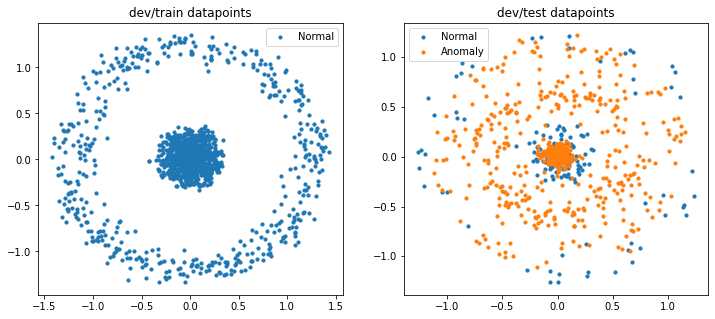
\includegraphics[width=\linewidth]{assets/pca.png}
    \caption{Distribution of dev samples after a 2-component PCA is performed.}
    \label{fig:pca}
\end{figure}
\begin{itemize}
	\item \textbf{PCA and KDE:} This approach yield unsatisfactory results. While some structure emerges while performing a PCA (as shown in Figure \ref{fig:pca}), the anomaly distribution seems to partially overlap the normal one making this method under-perform. Another reason why KDE fails is that, in order to represent meaningful information in our transformation, we have to increase significantly the resolution of our FFT or the components kept by PCA, incurring in the curse of dimensionality for the KDE.
	
	\item \textbf{PCA and DBSCAN:} This method performs well enough, reaching 0.85 of accuracy on the dev/test set. However, it requires a manual and finely grained fine-tuning to find hyperparameters that correctly separate areas with a high density of anomalous samples from areas with a lower one. This happens because the separation between these two regions is thin and variable. Parameters obtained by fine-tuning on the dev test did not work properly for the eval one, and of course a similar tuning for the latter is impossible as we do not know the distribution of normal and anomalous datapoints.
	\item  \textbf{f-ANOGAN:} This approach, without further tuning, reaches an AUC score of 0.68 on the dev set and 0.62 on the leaderboard.
	\item \textbf{VAE and KDE:} We incur in a similar problem as the one discussed above. In order to represent meaningful informations about the model we have to increase the size of the latent space. Doing so affects the performance of the downstream models yielding unsatisfactory results. Likelihoods of normal and anomalous samples are more or less the same and no conclusion can be drawn.
	\item \textbf{SVDD:} This approach proves unsatisfactory since both the one-class loss and soft-boundary one require the anomalies to fall outside of the of the hypersphere's boundary. Figure \ref{fig:pca} is a simple visualization showing this is not the case.

\end{itemize}

\section{Conclusions}
This challenge puts on display the limitations of classical machine learning approaches. The intricacies of this problem cannot be effectively summarized by low dimensional representations as they are not sufficient to make a distinction. On the other hand, increasing dimensionality is detrimental for these models. Generative deep learning models seem to be the way to go: 
While XXX outperforms other models, our analysis is rather limited by time and computational resources. Future works could evaluate different methods and architectures. A possible attempt we suggest is tuning the f-ANOGAN architecture to find one that works best with our dataset.

%% display bibliography at the end
\printbibliography
\end{document}